\documentclass[journal,12pt,twocolumn]{IEEEtran}

 \usepackage{setspace}
 \usepackage{gensymb}
 \usepackage{graphicx}

 \singlespacing

\graphicspath{ {/user/adarshsrivastava/desktop/Matrix Theory/Assignemnt_5} }
 \usepackage[cmex10]{amsmath}

 \usepackage{amsthm}
 \usepackage{hyperref}
 \usepackage{mathrsfs}
 \usepackage{txfonts}
 \usepackage{stfloats}
 \usepackage{bm}
 \usepackage{cite}
 \usepackage{cases}
 \usepackage{subfig}

 \usepackage{longtable}
 \usepackage{multirow}

 \usepackage{enumitem}
 \usepackage{mathtools}
 \usepackage{steinmetz}
 \usepackage{tikz}
 \usepackage{circuitikz}
 \usepackage{verbatim}
 \usepackage{tfrupee}
 \usepackage[breaklinks=true]{hyperref}

 \usepackage{tkz-euclide}

 \usetikzlibrary{calc,math}
 \usepackage{listings}
     \usepackage{color}                                            %%
     \usepackage{array}                                            %%
     \usepackage{longtable}                                        %%
     \usepackage{calc}                                             %%
     \usepackage{multirow}                                         %%
     \usepackage{hhline}                                           %%
     \usepackage{ifthen}                                           %%
     \usepackage{lscape}     
 \usepackage{multicol}
 \usepackage{chngcntr}

 \DeclareMathOperator*{\Res}{Res}

 \renewcommand\thesection{\arabic{section}}
 \renewcommand\thesubsection{\thesection.\arabic{subsection}}
 \renewcommand\thesubsubsection{\thesubsection.\arabic{subsubsection}}

 \renewcommand\thesectiondis{\arabic{section}}
 \renewcommand\thesubsectiondis{\thesectiondis.\arabic{subsection}}
 \renewcommand\thesubsubsectiondis{\thesubsectiondis.\arabic{subsubsection}}


 \hyphenation{op-tical net-works semi-conduc-tor}
 \def\inputGnumericTable{}                                 %%

 \lstset{
 %language=C,
 frame=single, 
 breaklines=true,
 columns=fullflexible
 }
 \begin{document}


 \newtheorem{theorem}{Theorem}[section]
 \newtheorem{problem}{Problem}
 \newtheorem{proposition}{Proposition}[section]
 \newtheorem{lemma}{Lemma}[section]
 \newtheorem{corollary}[theorem]{Corollary}
 \newtheorem{example}{Example}[section]
 \newtheorem{definition}[problem]{Definition}

 \newcommand{\BEQA}{\begin{eqnarray}}
 \newcommand{\EEQA}{\end{eqnarray}}
 \newcommand{\define}{\stackrel{\triangle}{=}}
 \bibliographystyle{IEEEtran}
 \providecommand{\mbf}{\mathbf}
 \providecommand{\pr}[1]{\ensuremath{\Pr\left(#1\right)}}
 \providecommand{\qfunc}[1]{\ensuremath{Q\left(#1\right)}}
 \providecommand{\sbrak}[1]{\ensuremath{{}\left[#1\right]}}
 \providecommand{\lsbrak}[1]{\ensuremath{{}\left[#1\right.}}
 \providecommand{\rsbrak}[1]{\ensuremath{{}\left.#1\right]}}
 \providecommand{\brak}[1]{\ensuremath{\left(#1\right)}}
 \providecommand{\lbrak}[1]{\ensuremath{\left(#1\right.}}
 \providecommand{\rbrak}[1]{\ensuremath{\left.#1\right)}}
 \providecommand{\cbrak}[1]{\ensuremath{\left\{#1\right\}}}
 \providecommand{\lcbrak}[1]{\ensuremath{\left\{#1\right.}}
 \providecommand{\rcbrak}[1]{\ensuremath{\left.#1\right\}}}
 \theoremstyle{remark}
 \newtheorem{rem}{Remark}
 \newcommand{\sgn}{\mathop{\mathrm{sgn}}}
 \providecommand{\abs}[1]{\left\vert#1\right\vert}
 \providecommand{\res}[1]{\Res\displaylimits_{#1}} 
 \providecommand{\norm}[1]{\left\lVert#1\right\rVert}
 %\providecommand{\norm}[1]{\lVert#1\rVert}
 \providecommand{\mtx}[1]{\mathbf{#1}}
 \providecommand{\mean}[1]{E\left[ #1 \right]}
 \providecommand{\fourier}{\overset{\mathcal{F}}{ \rightleftharpoons}}
 %\providecommand{\hilbert}{\overset{\mathcal{H}}{ \rightleftharpoons}}
 \providecommand{\system}{\overset{\mathcal{H}}{ \longleftrightarrow}}
 	%\newcommand{\solution}[2]{\textbf{Solution:}{#1}}
 \newcommand{\solution}{\noindent \textbf{Solution: }}
 \newcommand{\cosec}{\,\text{cosec}\,}
 \providecommand{\dec}[2]{\ensuremath{\overset{#1}{\underset{#2}{\gtrless}}}}
 \newcommand{\myvec}[1]{\ensuremath{\begin{pmatrix}#1\end{pmatrix}}}
 \newcommand{\mydet}[1]{\ensuremath{\begin{vmatrix}#1\end{vmatrix}}}
 \numberwithin{equation}{subsection}
 \makeatletter
 \@addtoreset{figure}{problem}
 \makeatother
 \let\StandardTheFigure\thefigure
 \let\vec\mathbf
 \renewcommand{\thefigure}{\theproblem}
 \def\putbox#1#2#3{\makebox[0in][l]{\makebox[#1][l]{}\raisebox{\baselineskip}[0in][0in]{\raisebox{#2}[0in][0in]{#3}}}}
      \def\rightbox#1{\makebox[0in][r]{#1}}
      \def\centbox#1{\makebox[0in]{#1}}
      \def\topbox#1{\raisebox{-\baselineskip}[0in][0in]{#1}}
      \def\midbox#1{\raisebox{-0.5\baselineskip}[0in][0in]{#1}}
 \vspace{3cm}
 \title{Assignment 5}
 \author{Adarsh Srivastava}
 \maketitle
 \newpage
 \bigskip
 %\renewcommand{\thefigure}{\theenumi}
 \renewcommand{\thetable}{\theenumi}
 The link to the solution is
 \begin{lstlisting}
  https://github.com/Adarsh1310/EE5609
 \end{lstlisting}
 \begin{abstract}
 This documents solves a problem based on circles.
 \end{abstract}
 \section{\textbf{Problem}}
Find the area of the region bounded by the circle $\bf{x}^{T}$ $\bf{x}$= 2 and \norm{\vec{x}-\myvec{2\\0}}=2.
 \section{\textbf{Solution}}
\vec{x}^{T}\vec{x}-2\vec(O)^{T}\vec{x}+\norm{\vec{O}}^2-\vec{r}^2=0\\
 $So from above equation we can say that,\\
 Circle 1:\\
 Equation of circle 1:\\
 \begin{align}
 \bf{x}^{T}\bf{x}= 2
 \end{align}
 radius=2\\
 point of origin as (0,0)\\ 
 Circle 2:\\
 Equation of circle 2:\\
\begin{align}
  \norm{\vec{x}-\myvec{2\\0}}^2\\
  {\vec{x}^{T}\vec{x}-2\myvec{2\\0}^T\vec{x}}+2-4=0\\
  {\vec{x}^{T}\vec{x}-\myvec{0\\4}^T\vec{x}}-2=0
  \end{align}
radius=2\\
point of origin as (2,0)\\
Subtracting equation 2.0.4 from 2.0.1\\
We get,
 \begin{align}
 \myvec{1&0}\vec{x}=0\\
 \vec{x} = \lambda \vec{m}, where \vec{m} = \myvec{0\\1}\\
 \vec{x} = \lambda \myvec{0\\1}\\
 \end{align}
 Substituting 2.0.7 in 2.0.1\\
 \begin{align}
  \vec{\lambda} = \sqrt{2}\myvec{0\\1}
 \end{align}
 \begin{figure}[h!]
	\centering
	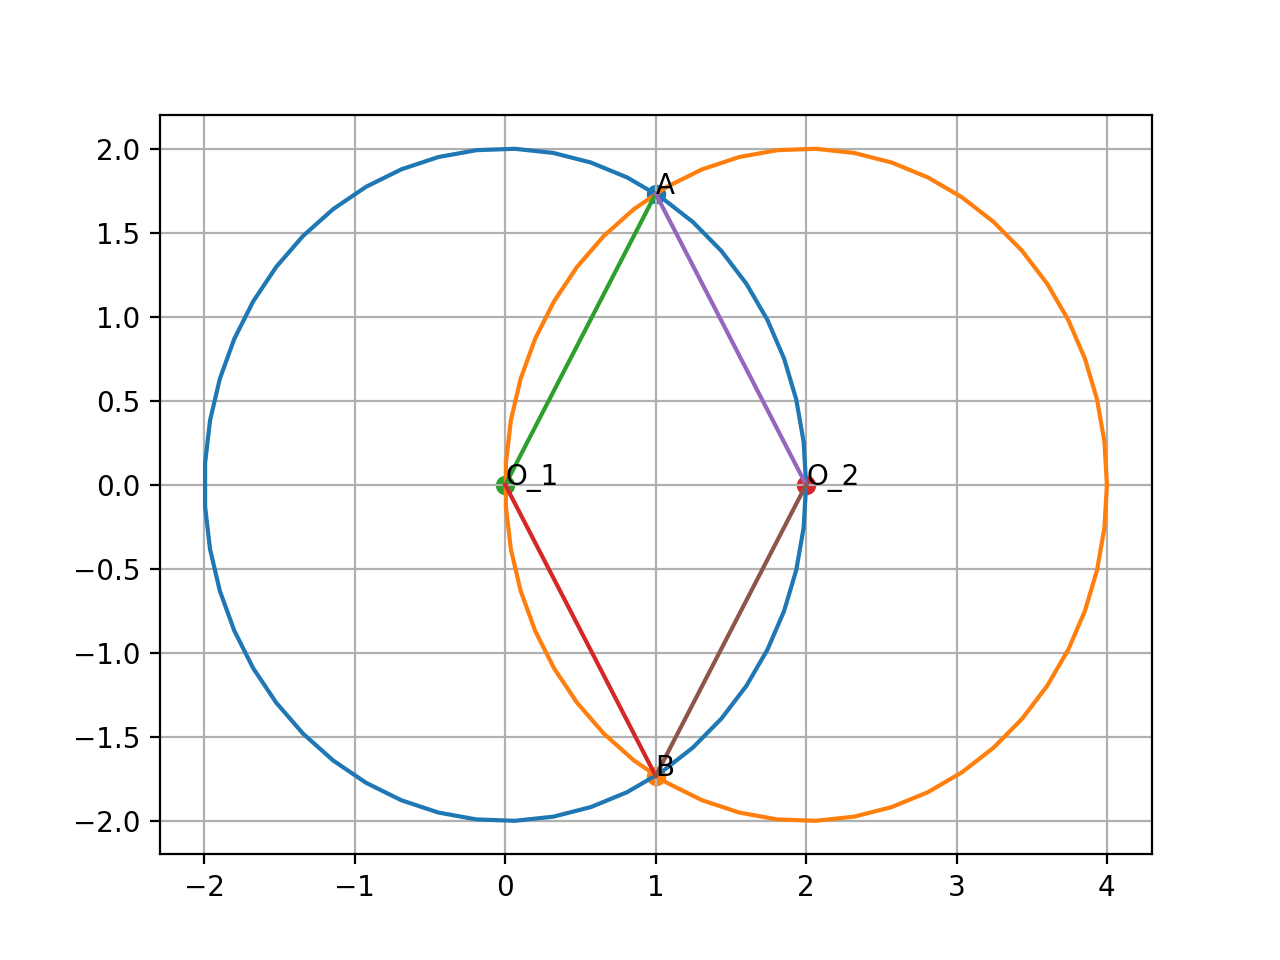
\includegraphics[width=\columnwidth]{Assignment_5.png}
	\caption{Figure depicting intersection points of circle}
	\label{myfig}
\end{figure}
 \\
 Now finding points of intersection:\\
 \\
Equation in general form is as follows:\\
 \begin{align}
 x^{2}+y^{2}=4\\
 (x-2)^{2}+y^{2}=4
 \end{align}
 Now Comparing equation 2.0.1 and 2.0.2:\\
 \\
 \begin{align}
 (x-2)^{2}+(4-x^{2})=4\\
 x^2+4-2x+4-x^2=4
 \end{align}
 x comes out to be 1\\ \\
 Now,Substituting the value of x in equation 2.0.1:\\
 y comes out to be \sqrt{3} and -\sqrt{3}\\ 
 $So the points of intersection of the two circles are $(1,\sqrt{3}) and(1,-\sqrt{3})$$\\ 
$Now to find the area inclosed between these circles we have to find the integral of these point w.r.t the circles.For this we need to find the area of segment $\bf{ABE}$ and double it to find the area of the entire overlapped region.\\ 
To find the area of segment ABE we need angle CDA as:\\$
Here,\\
$r=2 and $\theta=\angle CDA$$\\ 
$Now we have to find the angle\\ 
\sin \theta=\frac{\vec{AC}}{\vec{AD}}\\ 
\theta=30^{\circ}\\
\angle ADB=2*\theta\\
So,\angle ADB=60^{\circ}$\\
 \begin{align}
 \begin{multlined}
 Area=\frac{1}{2}(\frac{\angle ADB}{360}-\sin (\angle ADB))r^{2}\\
 $(Area of Sector-Area of Triangle)$
\end{multlined}\\
Area={\frac{1}{2}}(\frac{\pi}{3}-\sin 60)r^{2}\\
=\frac{1}{2}(\frac{4\pi}{3}-\sqrt{3})\\
Total area=2*Area\\
=\frac{4\pi}{3}-\sqrt{3}
\end{align}
 
 
  \end{document}